\begin{figure}[H]
  \centering
  \begin{subfigure}[b]{0.2\textwidth}
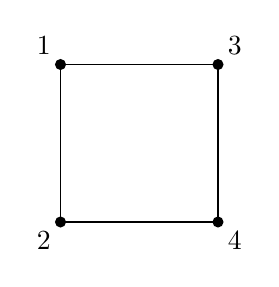
\begin{tikzpicture}
    % Define the length of the side of the triangle
    \def\side{1.}

    % Fill the equilateral triangle centered at (0,0)
    % Use \fill instead of \filldraw to avoid drawing the edge between 1 and 2
    %\fill[fill=yellow!40] (90: \side) -- (210: \side) -- (330: \side) -- cycle;
    
    % Draw the edges between the other two pairs of vertices
    %\draw (-\side, -\side) -- (\side, -\side); % Edge between vertices 2 and 3
   % \draw (\side, -\side) -- (\side, \side);  % Edge between vertices 3 and 1
   % \draw (\side, \side) -- (-\side, \side);
   % \draw (-\side, \side) -- (-\side, -\side);
   
    \filldraw[fill=white] (-\side, -\side) -- (\side, -\side) -- (\side, \side) -- (-\side, \side) -- (-\side, -\side) -- cycle;
    %\draw (-\side, -\side) -- (\side, \side);

    % Connect the center with all three vertices
    %\draw (0,0) -- (90: \side);
    
    % Fill the vertices with yellow circles (2pt)
    \fill (-\side, \side) circle (2pt);  % Vertex 1
    \fill (-\side, -\side) circle (2pt); % Vertex 2
    \fill (\side, \side) circle (2pt); % Vertex 3
    \fill (\side, -\side) circle (2pt);  % Vertex 4

    % Label the vertices and the center
    \node at (-\side, \side) [above left] {1};
    \node at (-\side, -\side) [below left] {2};
    \node at (\side, \side) [above right] {3};
    \node at (\side, -\side) [below right] {4};
\end{tikzpicture}
\caption{$\KK$.}
\end{subfigure}%
\quad
 \begin{subfigure}[b]{0.2\textwidth}
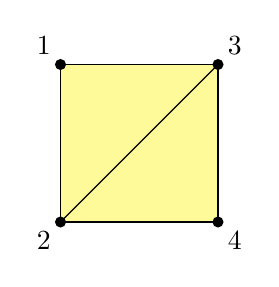
\begin{tikzpicture}
    % Define the length of the side of the triangle
    \def\side{1.}

    % Fill the equilateral triangle centered at (0,0)
    % Use \fill instead of \filldraw to avoid drawing the edge between 1 and 2
    %\fill[fill=yellow!40] (90: \side) -- (210: \side) -- (330: \side) -- cycle;
    
    % Draw the edges between the other two pairs of vertices
    %\draw (-\side, -\side) -- (\side, -\side); % Edge between vertices 2 and 3
   % \draw (\side, -\side) -- (\side, \side);  % Edge between vertices 3 and 1
   % \draw (\side, \side) -- (-\side, \side);
   % \draw (-\side, \side) -- (-\side, -\side);
   
    \filldraw[fill=yellow!40] (-\side, -\side) -- (\side, -\side) -- (\side, \side) -- (-\side, \side) -- (-\side, -\side) -- cycle;
    \draw (-\side, -\side) -- (\side, \side);

    % Connect the center with all three vertices
    %\draw (0,0) -- (90: \side);
    
    % Fill the vertices with yellow circles (2pt)
    \fill (-\side, \side) circle (2pt);  % Vertex 1
    \fill (-\side, -\side) circle (2pt); % Vertex 2
    \fill (\side, \side) circle (2pt); % Vertex 3
    \fill (\side, -\side) circle (2pt);  % Vertex 4

    % Label the vertices and the center
    \node at (-\side, \side) [above left] {1};
    \node at (-\side, -\side) [below left] {2};
    \node at (\side, \side) [above right] {3};
    \node at (\side, -\side) [below right] {4};
\end{tikzpicture}
\caption{$\LL$.}
\end{subfigure}%
\caption{The matrix $\Delta_{1, \text{up}}^{\KK, \LL}$ associated to these two complexes is dense.}
\label{fig:dense_example}
\end{figure}